\documentclass[11pt,a4paper]{article}


\usepackage[utf8]{inputenc}
\usepackage{graphicx}
\usepackage{amsmath}
\usepackage{amsfonts}
\usepackage{booktabs}
\usepackage{url}
\usepackage[margin=2.5cm, textwidth=15cm]{geometry}
\usepackage{listings}  
\usepackage{xcolor} % 可选：支持自定义代码颜色  
\lstset{  
    language=Python,  
    basicstyle=\ttfamily\footnotesize,  
    keywordstyle=\color{blue},  
    stringstyle=\color{red},  
    commentstyle=\color{gray},  
    numbers=left,  
    numberstyle=\tiny\color{gray},  
    stepnumber=1,  
    numbersep=5pt,  
    showstringspaces=false,  
    breaklines=true,  
    frame=single,  
    tabsize=4,  
    backgroundcolor=\color{white},  
    captionpos=b  
} 

\title{MSDM 5056 Lab 2: Small-World Networks}
\author{TANG,Yirui}
\date{}

\begin{document}

\maketitle

\section{Introduction}
\indent

This report investigates small-world networks using the Watts-Strogatz (WS) model. Small-world networks are characterized by simultaneously having a high clustering coefficient (local connectivity) and a short average path length (global connectivity). This unique combination, as observed in many real-world networks including social networks and neural networks, enables efficient information transfer while maintaining strong local clusters. The WS model elegantly demonstrates how these properties emerge from a simple rewiring process applied to a regular lattice. This lab generates small-world networks with 1000 nodes and constant average degree, then analyzes how their key properties vary with rewiring probability.

\section{Watts-Strogatz Model}

\subsection{Theoretical Background}
\indent

The Watts-Strogatz model (1998) provides a mathematical framework to explain the "six degrees of separation" phenomenon observed in social networks. The model starts with a regular ring lattice where each node connects to its $K$ nearest neighbors. Then, with probability $p$, each edge is rewired to connect to a randomly selected node. This single parameter $p$ smoothly interpolates between:

\begin{itemize}
    \item $p=0$: Regular lattice with high clustering coefficient $C(0)$ and long average path length $L(0) \sim N$
    \item $p=1$: Random graph with low clustering coefficient $C(0)/N$ and short average path length $L(1) \sim \ln N$
    \item $0 < p < 1$: Small-world network with both high clustering and short average path
\end{itemize}

The transition between these regimes reveals a crucial insight: only a few random connections (small $p$) are needed to dramatically reduce the average path length while preserving high clustering. In the WS model, the clustering coefficient can be approximated as:

\begin{equation}
C(p) \approx C(0)(1-p)^3
\end{equation}

where $(1-p)^3$ represents the probability that all three edges of a triangle remain intact after rewiring.


\subsection{Parameters and Implementation}
\indent

We generated Watts-Strogatz networks with the following parameters:
\begin{itemize}
    \item Network size: $N = 1000$ nodes
    \item Average degree: $K = 8$ (must be even for ring lattice formation)
    \item Rewiring probability range: $p \in [0.001, 1.0]$ (logarithmic scale)
    \item Samples per $p$: 10 networks (to average random fluctuations)
\end{itemize}

For each rewiring probability $p$, we:
\begin{enumerate}
    \item Generated 10 WS networks using the \texttt{nx.watts\_strogatz\_graph} function
    \item Calculated the average shortest path length $L(p)$ and clustering coefficient $C(p)$ for each network
    \item Normalized results by dividing by their values at $p=0$: $L(p)/L(0)$ and $C(p)/C(0)$
    \item Averaged these normalized values across all 10 samples
\end{enumerate}

The base regular lattice ($p=0$) had $L(0) = 62.9379$ and $C(0) = 0.6429$. For each $p$, we handled disconnected networks by computing metrics on the giant connected component. The algorithm used BFS-based shortest path calculation (\texttt{nx.average\_shortest\_path\_length}) for efficiency.

\subsection{Results and Analysis}

\begin{figure}[htbp]
  \centering
  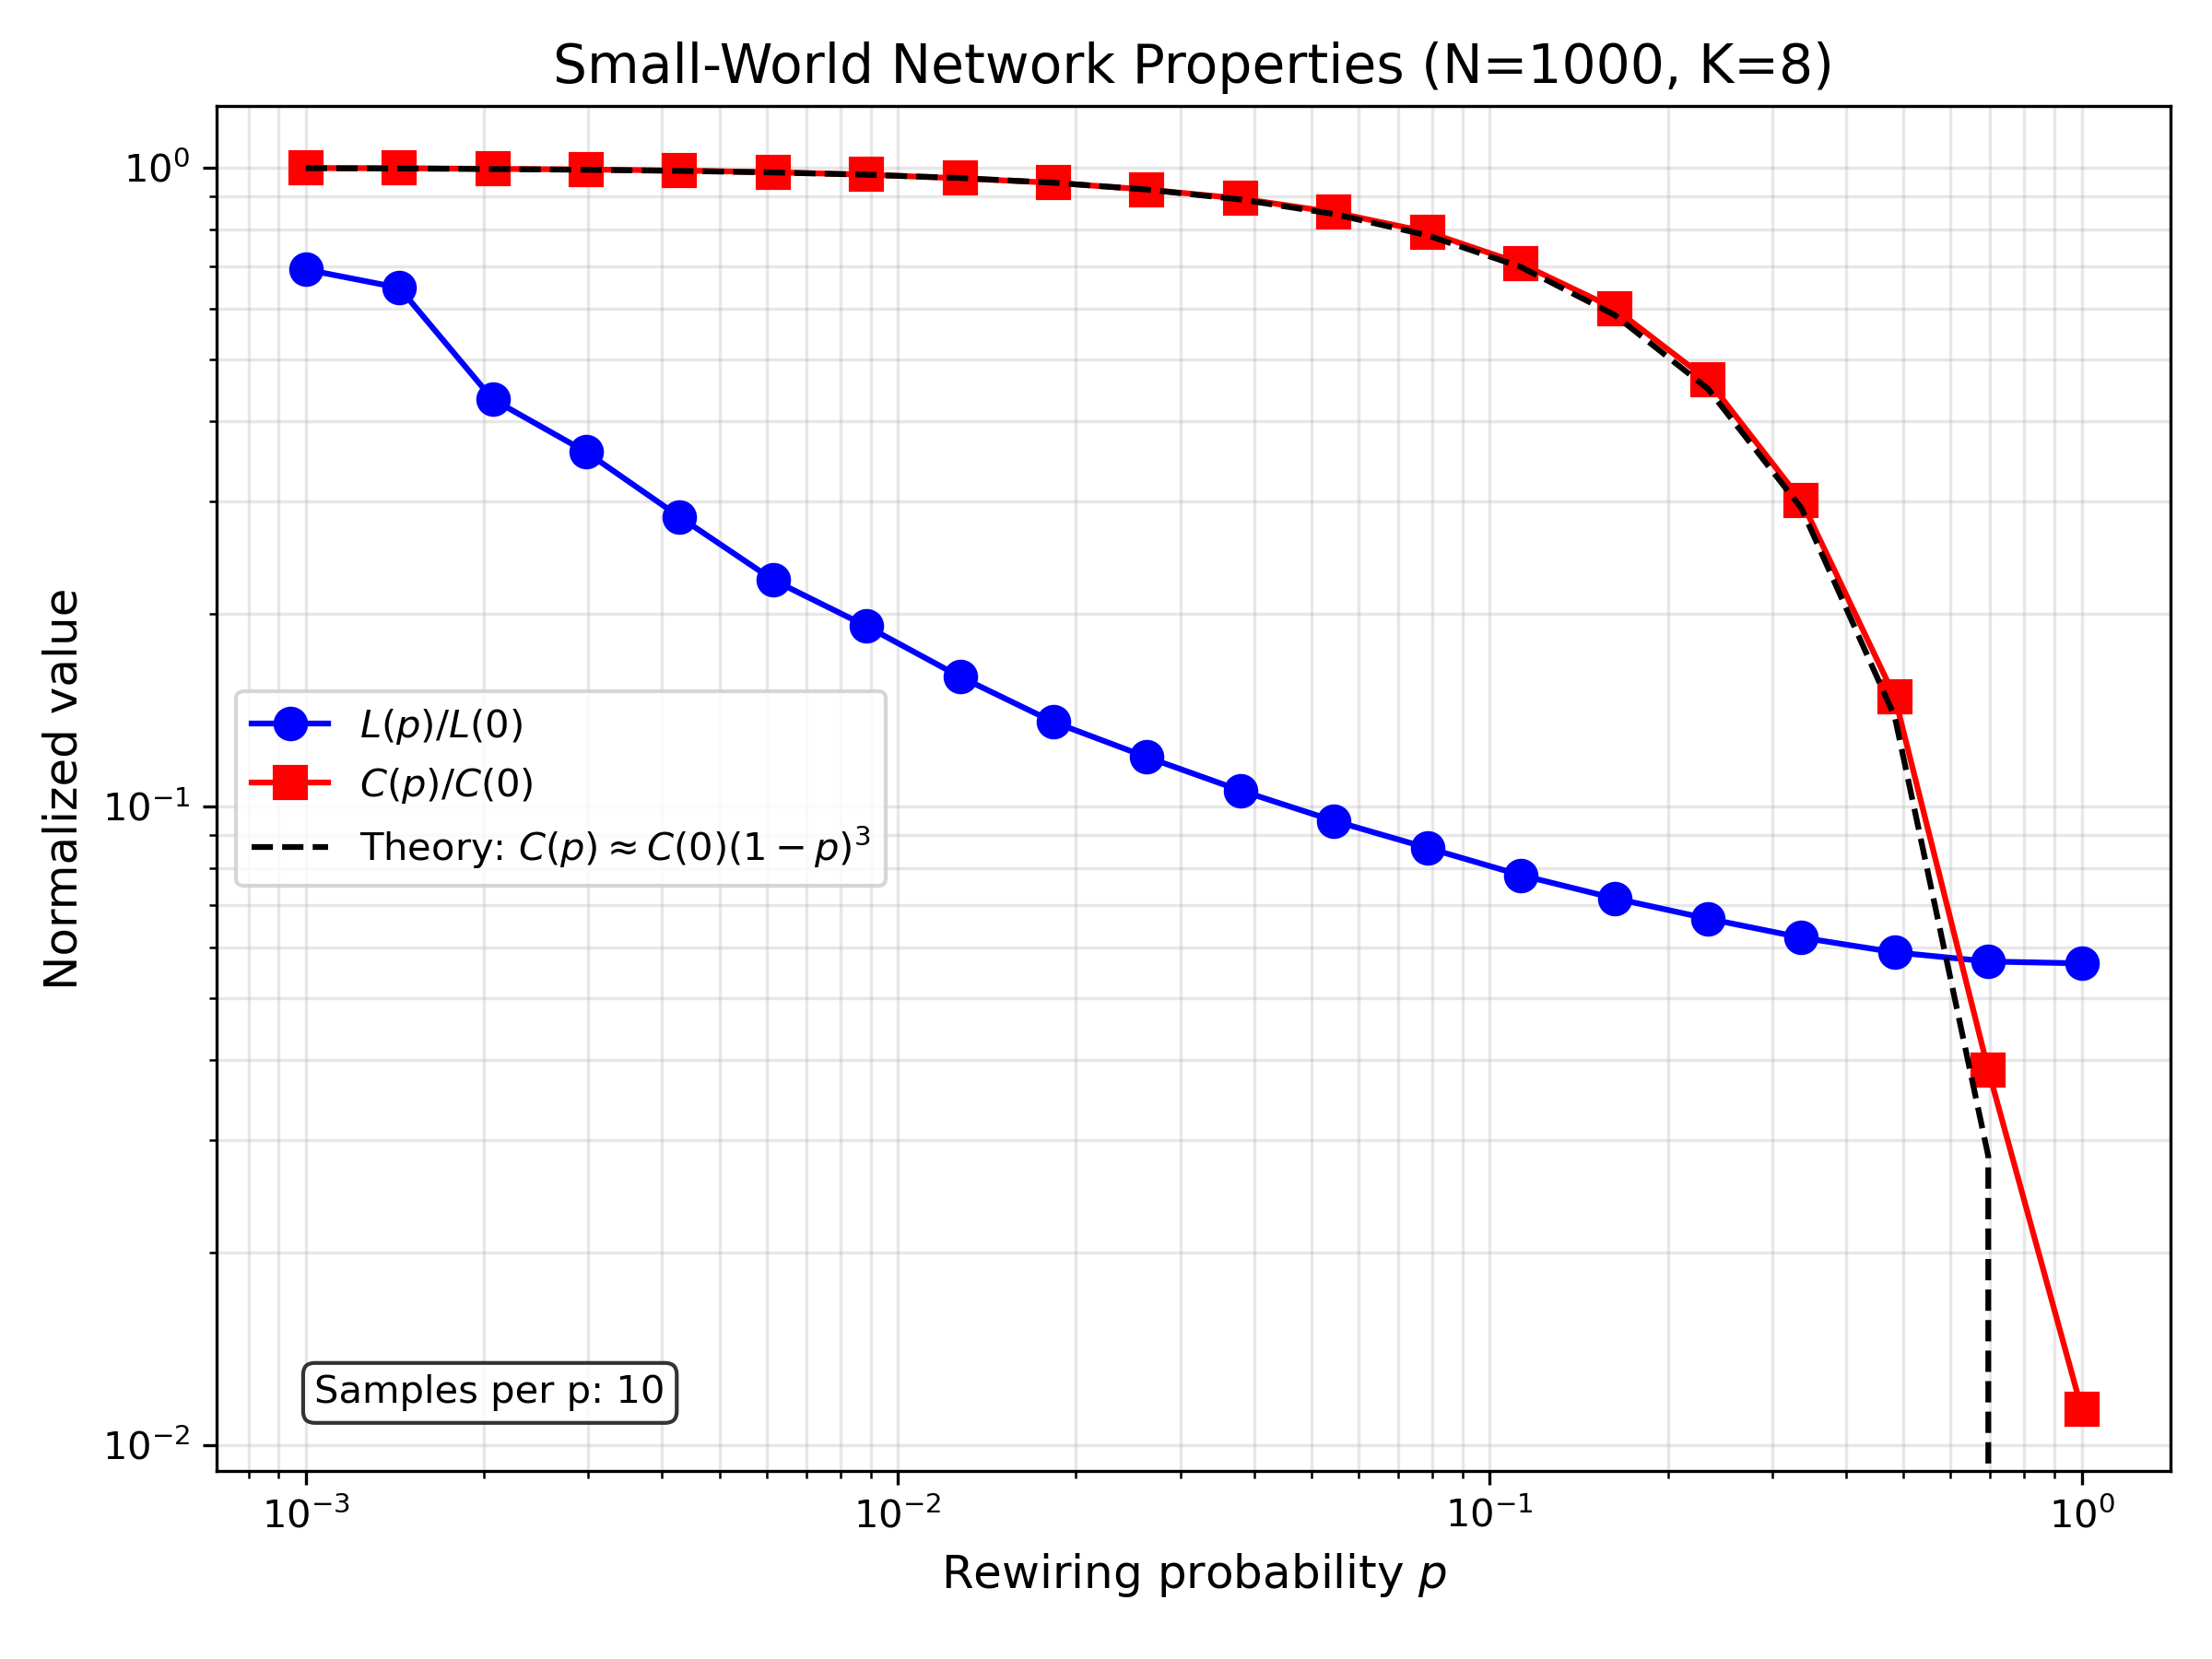
\includegraphics[width=0.8\textwidth]{small_world_crossover.png}
  \caption{Normalized average shortest path length $L(p)/L(0)$ (blue) and clustering coefficient $C(p)/C(0)$ (red) as functions of rewiring probability $p$. The black dashed line shows the theoretical approximation $C(p) \approx C(0)(1-p)^3$.}
  \label{fig:small_world}
\end{figure}

Figure~\ref{fig:small_world} displays the key result of this experiment. The plot reveals the characteristic crossover behavior of small-world networks:

\begin{enumerate}
    \item \textbf{Clustering coefficient}: $C(p)/C(0)$ decreases gradually following the theoretical curve $C(p) \approx C(0)(1-p)^3$, indicating that local clustering remains robust even with moderate rewiring.
    
    \item \textbf{Average path length}: $L(p)/L(0)$ drops dramatically with even small values of $p$. At $p=0.01$, the path length is already less than 20\% of its original value.
    
    \item \textbf{Small-world region}: Between $p \approx 0.01$ and $p \approx 0.1$, the network simultaneously maintains high clustering ($C(p)/C(0) > 0.5$) and short path lengths ($L(p)/L(0) < 0.2$).
\end{enumerate}

This transition occurs because random rewiring creates "shortcuts" that connect distant parts of the network, dramatically improving global connectivity while minimally affecting local clustering. The theoretical approximation for $C(p)$ is accurate for small $p$ but underestimates the actual clustering coefficient for larger $p$ values because it doesn't account for new triangles formed during rewiring.

% \section{Computational Challenges and Optimization}

\subsection{Implementation Details}
\indent

The most significant computational challenge was efficiently calculating the average shortest path length for networks with 1000 nodes. The naive approach using Floyd-Warshall algorithm (\texttt{nx.floyd\_warshall\_numpy}) would require $O(N^3)$ time and $O(N^2)$ memory, becoming prohibitively expensive for large networks.

Our solution used:
\begin{enumerate}
    \item \textbf{BFS-based shortest paths}: The \texttt{nx.average\_shortest\_path\_length} function uses breadth-first search, with complexity $O(N(N+E))$, which is significantly faster for sparse networks.
    \item \textbf{Giant component handling}: For small $p$ values, networks might have minor disconnected components. We identified the largest connected component using \texttt{nx.connected\_components} before path length calculation.
    \item \textbf{Sample averaging}: Computing metrics over 10 samples per $p$ value smoothed statistical fluctuations while remaining computationally feasible.
\end{enumerate}

The entire experiment completed in approximately 42 seconds on a standard laptop, demonstrating the efficiency of these optimizations.

\section{Conclusion}
\indent

This experiment successfully demonstrated the small-world phenomenon as described by Watts and Strogatz. Our results confirm that only a small fraction of random connections (1-10\% rewiring probability) is sufficient to transform a regular lattice into a small-world network that maintains high clustering while dramatically reducing average path lengths.

These findings have profound implications for understanding real-world networks. Many naturally occurring systems, from neural networks to social networks, exhibit small-world properties that optimize the trade-off between local specialization (high clustering) and global integration (short paths). The Watts-Strogatz model elegantly explains how this structure can emerge through simple mechanisms.

Future work could investigate more realistic small-world models that incorporate geographical constraints or hierarchical organization, as suggested by Kleinberg's navigable small-world model. These extensions would better capture the navigability properties observed in actual social networks.

\section{Python Source Code}  


\vspace{0.5em}  
Below is the full Python code used for this lab report.  

\begin{lstlisting}[language=Python,caption={Complete Python code for Lab 2}]  
    
import numpy as np
import matplotlib.pyplot as plt
import networkx as nx
import time

# Parameters
N, K = 1000, 8  # Network size and degree (must be even)
trials = 10     # Number of samples to average for each p
p_values = np.logspace(-3, 0, 20)  # Rewiring probability from 0.001 to 1.0
ws = nx.watts_strogatz_graph

# Initialize arrays for normalized results
L_norm = np.zeros(len(p_values))
C_norm = np.zeros(len(p_values))

# First create base network (p=0) to get L(0) and C(0)
base_net = ws(N, K, 0, seed=3042)
L0 = nx.average_shortest_path_length(base_net)
C0 = nx.average_clustering(base_net)
print(f"Base network (p=0): L(0)={L0:.4f}, C(0)={C0:.4f}")

# Process each rewiring probability
start_time = time.time()
for i, p in enumerate(p_values):
    # Print progress every 10 iterations
    if i % 10 == 0:
        print(f"Processing p={p:.4f} ({i+1}/{len(p_values)})")
    
    L_sum, C_sum = 0, 0
    
    for t in range(trials):
        # Generate WS network
        G = ws(N, K, p, seed = 3042+t)
        
        # Handle disconnected graphs by using the giant component
        if not nx.is_connected(G):
            giant = max(nx.connected_components(G), key=len)
            G = G.subgraph(giant).copy()
        
        # Calculate metrics
        L = nx.average_shortest_path_length(G)
        C = nx.average_clustering(G)
        
        L_sum += L
        C_sum += C
    
    # Normalize by base values
    L_norm[i] = (L_sum/trials) / L0
    C_norm[i] = (C_sum/trials) / C0

# Calculate theoretical clustering coefficient
theory_C = 0.75 * (K-2)/(K-1) * (1-p_values)**3 / C0

# Plot results
plt.figure(figsize=(8, 6))
plt.loglog(p_values, L_norm, 'bo-', markersize=8, label=r'$L(p)/L(0)$')
plt.loglog(p_values, C_norm, 'rs-', markersize=8, label=r'$C(p)/C(0)$')
plt.loglog(p_values, theory_C, 'k--', linewidth=1.5, 
           label=r'Theory: $C(p) \approx C(0)(1-p)^3$')

# Chart formatting
plt.xlabel('Rewiring probability $p$', fontsize=12)
plt.ylabel('Normalized value', fontsize=12)
plt.title(f'Small-World Network Properties (N={N}, K={K})', fontsize=14)
plt.grid(True, which="both", ls="-", alpha=0.3)
plt.legend(loc='best')

# Add annotation about sample size
plt.annotate(f'Samples per p: {trials}', xy=(0.05, 0.05), xycoords='axes fraction',
             fontsize=10, bbox=dict(boxstyle="round,pad=0.3", facecolor='white', alpha=0.8))

plt.tight_layout()
plt.savefig('small_world_crossover.png', dpi=300)
plt.show()

# Print completion message
print(f"Completed in {time.time() - start_time:.1f} seconds")
print("Small-world behavior observed where:")
print(f"- High clustering (C(p)/C(0) > 0.5) occurs for p < {p_values[np.where(C_norm > 0.5)[0][-1]]:.4f}")
print(f"- Short path lengths (L(p)/L(0) < 0.2) occur for p > {p_values[np.where(L_norm < 0.2)[0][0]]:.4f}")

\end{lstlisting}  

\end{document}
```